\documentclass[12pt]{scrartcl}

\usepackage[T1]{fontenc}
\usepackage[utf8]{inputenc}
\usepackage{amsmath}
\usepackage{amsfonts}
\usepackage{amssymb}
\usepackage{amsbsy}
\usepackage{graphicx}
\usepackage{float}
\usepackage{array}
\usepackage{booktabs}
\usepackage{multirow}
\usepackage{bm}
\usepackage{verbatim}
\usepackage[english]{babel}
\usepackage{color}
\usepackage{url}
\usepackage{fancybox}
\usepackage[stable]{footmisc}
\usepackage[format=plain,labelfont=bf]{caption}
\usepackage{fancyhdr}
\usepackage{natbib}
\usepackage{calc}
\usepackage{textcomp}
\usepackage[pdftex,pdfborder={0 0 0}]{hyperref}
\usepackage{pdfpages}
\usepackage{tikz}
\usetikzlibrary{shapes,backgrounds,fit,positioning,arrows,positioning,decorations.pathmorphing,decorations.pathreplacing,backgrounds}
\usepackage{accents}

\renewcommand*{\familydefault}{\sfdefault}

% Margins
\addtolength{\textheight}{1.0cm}
\addtolength{\oddsidemargin}{-0.5cm}
\addtolength{\evensidemargin}{-0.5cm}
\addtolength{\textwidth}{1.0cm}
\parindent=0em

% New math commands
\newcommand{\overbar}[1]{\mkern 1.5mu\overline{\mkern-1.5mu#1\mkern-1.5mu}\mkern 1.5mu}
\DeclareMathOperator{\diag}{diag}
\DeclareMathOperator{\Diag}{Diag}
\DeclareMathOperator{\tr}{tr}
\DeclareMathOperator{\var}{var}
\DeclareMathOperator{\Cov}{Cov}
\DeclareMathOperator{\Cor}{Cor}
\newcommand\independent{\protect\mathpalette{\protect\independenT}{\perp}}
\def\independenT#1#2{\mathrel{\setbox0\hbox{$#1#2$}%
\copy0\kern-\wd0\mkern4mu\box0}}

% Appropriate font for \mathcal{}
\DeclareSymbolFont{cmmathcal}{OMS}{cmsy}{m}{n}
\DeclareSymbolFontAlphabet{\mathcal}{cmmathcal}

% Set subscript and superscripts positions
\everymath{
\fontdimen13\textfont2=5pt
\fontdimen14\textfont2=5pt
\fontdimen15\textfont2=5pt
\fontdimen16\textfont2=5pt
\fontdimen17\textfont2=5pt
}

% Bibliography style
\setlength{\bibsep}{1pt}

% Part
\renewcommand\partheadstartvskip{\clearpage\null\vfil}
\renewcommand\partheadmidvskip{\par\nobreak\vskip 20pt\thispagestyle{empty}}
\renewcommand\partheadendvskip{\vfil\clearpage}
\renewcommand\raggedpart{\centering}

\begin{document}
\title{Filter banks localization}
\author{Benjamin Ménétrier}
\date{Last update: \today}

\thispagestyle{empty}

\maketitle
\begin{center}
Copyright \copyright 2025: Meteorologisk Institutt
\end{center}

%\tableofcontents

\section{EnVar formulation}

\subsection{Standard EnVar formulation}
For an ensemble $N$ backgrounds $\left\{\mathbf{x}^1,\dots,\mathbf{x}^N\right\}$, with $\mathbf{x}^k \in \mathbb{R}^n$, the standard EnVar formulation is given by:
\begin{align}
\label{eq:envar}
\mathbf{B} = \mathbf{X}\mathbf{X}^\mathrm{T} \circ \mathbf{L}
\end{align}
where:
\begin{itemize}
\item $\mathbf{B} \in \mathbb{R}^{n \times n}$ is the resulting background error covariance.
\item $\mathbf{X} \in \mathbb{R}^{n \times N}$ contains the normalized ensemble perturbations:
\begin{align}
X_{ij} = \frac{1}{\sqrt{N-1}} \left(x^j_i - \langle x_i \rangle\right)
\end{align}
with $\langle x_i \rangle$ denoting the ensemble mean:
\begin{align}
\langle x_i \rangle = \frac{1}{N} \sum_{j=1}^N x^j_i
\end{align}
\item $\mathbf{L} \in \mathbb{R}^{n \times n}$ is the localization matrix.
\item $\circ$ denotes a Schur product between matrices (element-by-element).
\end{itemize}
The square-root expression of \eqref{eq:envar}, transforming the control vector $\mathbf{v} \in \mathbb{R}^m$ into a control increment $\delta \mathbf{x} \in \mathbb{R}^n$, is given by:
\begin{align}
\delta \mathbf{x} = \sum_{j=1}^N \mathbf{X}_{:j} \circ \left(\mathbf{U} \mathbf{v}_j\right)
\end{align}
where:
\begin{itemize}
\item $\mathbf{X}_{:j} \in \mathbb{R}^n$ is the j$^\text{th}$ column of $\mathbf{X}$
\item $\mathbf{U} \in \mathbb{R}^{n \times m}$ is a square-root of the localization $\mathbf{L}$ such that $\mathbf{U} \mathbf{U}^\mathrm{T} = \mathbf{L}$.
\item $\mathbf{v}_j \in \mathbb{R}^{m/N}$ is the j$^\text{th}$ subvector of $\mathbf{v}$.
\end{itemize}

\subsection{Generalized EnVar formulation}
The standard EnVar formulation can be generalized by introducing two linear transforms $\mathbf{F} \in \mathbb{R}^{n \times \widehat{n}}$ and $\mathbf{F}^\dag \in \mathbb{R}^{\widehat{n} \times n}$:
\begin{align}
\widehat{\mathbf{B}} & = \mathbf{F} \left(\left(\mathbf{F}^\dag \mathbf{X}\right) \left(\mathbf{F}^\dag \mathbf{X}\right)^\mathrm{T} \circ \widehat{\mathbf{L}}\right) \mathbf{F}^\mathrm{T} \\
\delta \mathbf{x} & = \mathbf{F} \sum_{j=1}^N \left(\mathbf{F}^\dag \mathbf{X}_{:j}\right) \circ \left(\widehat{\mathbf{U}} \widehat{\mathbf{v}}_j\right)
\end{align}
where: 
\begin{itemize}
\item $\widehat{\mathbf{L}} \in \mathbb{R}^{\widehat{n} \times \widehat{n}}$ is the localization matrix in the transformed space.
\item $\widehat{\mathbf{U}} \in \mathbb{R}^{n \times \widehat{m}}$ is a square-root of the localization $\widehat{\mathbf{L}}$ such that $\widehat{\mathbf{U}} \widehat{\mathbf{U}}^\mathrm{T} = \widehat{\mathbf{L}}$.
\item $\widehat{\mathbf{v}}_j \in \mathbb{R}^{\widehat{m}/N}$ is the j$^\text{th}$ subvector of $\widehat{\mathbf{v}} \in \mathbb{R}^{\widehat{m}}$.
\end{itemize}
Let's analyse the asymptotic values if the ensemble size grows to infinity:
\begin{itemize}
\item The localization matrices $\mathbf{L}$ and $\widehat{\mathbf{L}}$ should converge to $\mathbf{1}_n$ and $\mathbf{1}_{\widehat{n}}$, respectively, where $\mathbf{1}_n \in \mathbb{R}^{n \times n}$ is a matrix filled with 1.
\item As a consequence:
\begin{align}
\lim_{N \rightarrow \infty} \mathbf{B} & = \mathbf{X} \mathbf{X}^\mathrm{T} \\
\lim_{N \rightarrow \infty} \widehat{\mathbf{B}} & = \left(\mathbf{F} \mathbf{F}^\dag \mathbf{X}\right) \left(\mathbf{F} \mathbf{F}^\dag \mathbf{X}\right)^\mathrm{T}
\end{align}
\item To ensure consistency, linear transforms $\mathbf{F}$ and $\mathbf{F}^\dag$ should not have an impact on the asymptotic background error covariance:
\begin{align}
\lim_{N \rightarrow \infty} \mathbf{B} = \lim_{N \rightarrow \infty} \widehat{\mathbf{B}}
\end{align}
so
\begin{align}
\mathbf{F} \mathbf{F}^\dag \mathbf{X} = \mathbf{X}
\end{align}
Thus, $\mathbf{F}^\dag$ should be a right-inverse of $\mathbf{F}$ in the ensemble perturbations space.
\end{itemize}

The content of $\mathbf{F}$ and $\mathbf{F}^\dag$ can be very diverse:
\begin{itemize}
\item A change of variables: for instance towards a better-suited humidity variable.
\item A inverse balance operator as in \citet{clayton_2012}, where the localization is applied on unbalanced variables and the balance operator is finally applied to get the increment.
\item A change of resolution as in \citet{kleist_2014a}, where the ensemble resolution is lower than the final increment one. In this case, $\mathbf{F}$ is an interpolation from low to high resolution, and the low-resolution perturbations $\mathbf{X}_\mathrm{LR}$ can be thought as the application of a coarsening operator $\mathbf{F}^\dag$ on virtual high-resolution perturbations $\mathbf{X}_\mathrm{HR}$ representing the same field:
\begin{align}
\mathbf{F} \mathbf{X}_\mathrm{LR} = \mathbf{F} \mathbf{F}^\dag \mathbf{X}_\mathrm{HR} = \mathbf{X}_\mathrm{HR}
\end{align}
\end{itemize}

\section{Filter banks localization}

\subsection{The band-pass framework}
We define two series of $P$ linear transforms:
\begin{itemize}
\item the band-pass filters $\left\{\mathbf{H}_1,\dots,\mathbf{H}_P\right\}$, where $\mathbf{H}_p \in \mathbb{R}^{\widehat{n}_p \times n}$,
\item the interpolators $\left\{\mathbf{S}_1,\dots,\mathbf{S}_P\right\}$, where $\mathbf{S}_p \in \mathbb{R}^{n \times \widehat{n}_p}$,
\end{itemize}
where $\widehat{n}_p$ is the space size of component $p$. For each component, $\mathbf{S}_p \mathbf{H}_p \in \mathbb{R}^{n \times n}$ can be seen as the band-pass filter $p$ expressed at full resolution.\\
$  $\\
Formally, the linear transform $\mathbf{F}^\dag$ is defined as
\begin{align}
\mathbf{F}^\dag = \left( \begin{array}{c}
\mathbf{H}_1 \\
\mathbf{H}_2 \\
\vdots \\
\mathbf{H}_P
\end{array}
\right)
\end{align}
and its left-inverse as:
\begin{align}
\mathbf{F} = \left(\mathbf{S}_1 \mathbf{S}_2 \dots \mathbf{S}_{P}\right)
\end{align}
Thus, $\mathbf{F} \mathbf{F}^\dag$ is the sum of the band-pass filters expressed at full resolution:
\begin{align}
\mathbf{F} \mathbf{F}^\dag = \sum_{p=1}^P \mathbf{S}_p \mathbf{H}_p
\end{align}
and the size of the decomposition space (i.e. the number of rows of $\mathbf{F}^\dag$) is the sum of all the sizes of the components:
\begin{align}
\widehat{n} = \sum_{p=1}^P n_p
\end{align}
For $1 \le p \le P-1$, the band-pass filters $\mathbf{H}_p$ are defined freely, but to ensure that $\mathbf{F} \mathbf{F}^\dag = \mathbf{I}_n$, the last band-pass filter $\mathbf{H}_P$ is defined as the complement of the sum of all the previous band-pass filters interpolated at full resolution:
\begin{align}
\label{eq:bp1}
\mathbf{H}_P = \mathbf{I}_n - \sum_{p=1}^{P-1} \mathbf{S}_p \mathbf{H}_p
\end{align}
As a consequence for the last component $P$:
\begin{itemize}
\item the space size is $\widehat{n}_P = n$
\item the interpolator is $\mathbf{S}_P = \mathbf{I}_n$
\end{itemize}
We also define the filtered components $\widehat{\mathbf{x}}_p \in \mathbb{R}^{\widehat{n}_p}$ as:
\begin{align}
\label{eq:bp2}
\widehat{\mathbf{x}}_p = \mathbf{H}_p \mathbf{x}
\end{align}
where $\mathbf{x}$ is the input vector.

\subsection{Recursive construction}
In this section, we build the band-pass filters $\mathbf{H}_p$ recursively from a series of $P-1$ filters $\left\{\mathbf{G}_1,\dots,\mathbf{G}_{P-1}\right\}$, where $\mathbf{G}_p \in \mathbb{R}^{\widehat{n}_p \times n}$:
\begin{itemize}
\item The initial residual is given by the input state: $\overline{\mathbf{x}}_0 = \mathbf{x}$
\item At each iteration $1 \le p \le P-1$:
\begin{itemize}
\item The filter $\mathbf{G}_p$ is applied to the previous residual $\overline{\mathbf{x}}_{p-1} \in \mathbb{R}^n$ to produce the new filtered component $\widehat{\mathbf{x}}_p \in \mathbb{R}^{\widehat{n}_p}$:
\begin{align}
\label{eq:lp1}
\widehat{\mathbf{x}}_p = \mathbf{G}_p \overline{\mathbf{x}}_{p-1}
\end{align}
\item The new residual is computed from $\widehat{\mathbf{x}}_p$, interpolated at full resolution with $\mathbf{S}_p$:
\begin{align}
\label{eq:lp2}
\overline{\mathbf{x}}_p & = \overline{\mathbf{x}}_{p-1} - \mathbf{S}_p \widehat{\mathbf{x}}_p \\
& = \left(\mathbf{I}_n - \mathbf{S}_p \mathbf{G}_p\right) \overline{\mathbf{x}}_{p-1}
\end{align}
\end{itemize}
\end{itemize}
This construction can be illustrated as follows:
\begin{center}
\begin{tikzpicture}[scale=0.8,transform shape,auto,>=latex',line width=1pt]
\tikzstyle{block} = [draw, shape=rectangle, minimum height=0.8cm, minimum width=3.0cm]
\tikzstyle{branch}=[fill,shape=circle,minimum size=5pt,inner sep=0pt]

% Input
\node at (-2.5,0) (input) {$\mathbf{x}$};

% Filter 1
\node [block, right of=input, node distance=3.0cm] (F1) {$\mathbf{G}_1$};
\node [right of=F1, node distance=2.7cm, yshift=-0.02cm] (F1x) {$\widehat{\mathbf{x}}_1$};
\node [block, below of=F1, node distance=1.0cm] (ImF1) {$\mathbf{I}_n - \mathbf{S}_1 \mathbf{G}_1$};
\node [right of=ImF1, node distance=2.7cm, yshift=-0.02cm] (ImF1x) {$\overline{\mathbf{x}}_1$};
\path (input) -- coordinate(branch1) (F1);
\draw[->] (input) -- (F1);
\draw[->] (F1) -- ([yshift=0.02cm]F1x.west);
\draw[->] (ImF1) -- ([yshift=0.02cm]ImF1x.west);
\draw[->] (branch1) node[branch] {} |- (ImF1);

% Filter 2
\node [block, right of=ImF1, node distance=5.8cm] (F2) {$\mathbf{G}_2$};
\node [right of=F2, node distance=2.7cm, yshift=-0.02cm] (F2x) {$\widehat{\mathbf{x}}_2$};
\node [block, below of=F2, node distance=1.0cm] (ImF2) {$\mathbf{I}_n - \mathbf{S}_2 \mathbf{G}_2$};
\node [right of=ImF2, node distance=2.7cm, yshift=-0.02cm] (ImF2x) {$\overline{\mathbf{x}}_2$};
\path (ImF1x) -- coordinate(branch2) (F2);
\draw[->] (ImF1x) -- (F2);
\draw[->] (F2) -- ([yshift=0.02cm]F2x.west);
\draw[->] (ImF2) -- ([yshift=0.02cm]ImF2x.west);
\draw[->] (branch2) node[branch] {} |- (ImF2);

% Etc
\node [right of=ImF2x, node distance=2.0cm] (dots1) {\dots};
\node [below of=dots1, node distance=1.0cm] (dots2) {\dots};
\path (ImF2x) -- coordinate(branch3) (dots1);
\draw[->] (ImF2x) -- (dots1);
\draw[->] (branch3) node[branch] {} |- (dots2);

\end{tikzpicture}
\end{center}

Integrating recursively, the residual at iteration $p$ becomes:
\begin{align}
\label{eq:lp3}
\overline{\mathbf{x}}_p & = \left(\mathbf{I}_n - \mathbf{S}_p \mathbf{G}_p\right) \left(\mathbf{I}_n - \mathbf{S}_{p-1} \mathbf{G}_{p-1}\right) \dots \left(\mathbf{I}_n - \mathbf{S}_1 \mathbf{G}_1\right) \mathbf{x} \nonumber \\
& = \displaystyle \prod_{q=1}^p \left(\mathbf{I}_n - \mathbf{S}_q \mathbf{G}_q\right) \mathbf{x}
\end{align}
and from \eqref{eq:lp1}, we obtain the filtered component at iteration $p$:
\begin{align}
\label{eq:lp4}
\widehat{\mathbf{x}}_p & = \mathbf{G}_p \prod_{q=1}^{p-1} \left(\mathbf{I}_n - \mathbf{S}_q \mathbf{G}_q\right) \mathbf{x}
\end{align}

Combining equations \eqref{eq:bp2} with \eqref{eq:lp4}, we get an equivalence between $\mathbf{H}_p$ and $\mathbf{G}_p$ for $1 \le p \le P-1$:
\begin{align}
\label{eq:band_pass_filter}
\mathbf{H}_p = \mathbf{G}_p \prod_{q=1}^{p-1} \left(\mathbf{I}_n - \mathbf{S}_q \mathbf{G}_q\right)
\end{align}
The last filtered component $\widehat{\mathbf{x}}_P$ is actually given by the last residual $\overline{\mathbf{x}}_{P-1}$
\begin{align}
\widehat{\mathbf{x}}_P = \mathbf{H}_P \mathbf{x} = \overline{\mathbf{x}}_{P-1}
\end{align}
So equation \eqref{eq:lp3} gives another expression of equation \eqref{eq:bp1}:
\begin{align}
\mathbf{H}_P = \prod_{q=1}^{P-1} \left(\mathbf{I}_n - \mathbf{S}_q \mathbf{G}_q\right)
\end{align}

\subsection{Low-pass, band-pass and high-pass filters}
The filters $\mathbf{G}_p$ can be:
\begin{itemize}
\item either low-pass filters, with $\widehat{n}_p$ increasing up to $\widehat{n}_P = n$,
\item or high-pass filters, with $\widehat{n}_p$ decreasing from $\widehat{n}_1 = n$.
\end{itemize}
%TODO: detail et illustration

\subsection{High-pass filters built from low-pass filters}
Often in practice, only low-pass filters are actually implemented, through a diffusion process or an equivalent smoother. However, the high-pass filter $\mathbf{G}^h_p \in \mathbb{R}^{\widehat{n}^l_p \times n}$ can be built as the complement of the low-pass filter $\mathbf{G}^l_{P-p} \in \mathbb{R}^{\widehat{n}^l_{P-p} \times n}$:
\begin{align}
\mathbf{G}^h_p = \mathbf{I}_n - \mathbf{S}^l_p \mathbf{G}^l_p
\end{align}
But we should notice that the filters sizes are different:
\begin{itemize}
\item For the low-pass filter: $\widehat{n}^l_p$ can be lower than $n$,
\item For the high-pass filter: $\widehat{n}^h_p = n$ necessarily, so $\mathbf{S}^h_p = \mathbf{I}_n$
\end{itemize}

Updating equation \eqref{eq:band_pass_filter}, the band-pass filter $\mathbf{H}^h_p$ corresponding to the high-pass filters is given for $1 \le p \le P-1$ by:
\begin{align}
\label{eq:band_pass_filter_hp}
\mathbf{H}^h_p & = \mathbf{G}^h_p \prod_{q=1}^{p-1} \left(\mathbf{I}_n - \mathbf{G}^h_q\right) \nonumber \\
& = \left(\mathbf{I}_n - \mathbf{S}^l_{P-p} \mathbf{G}^l_{P-p}\right) \prod_{q=1}^{p-1} \mathbf{S}^l_{P-q} \mathbf{G}^l_{P-q}
\end{align}

Figure \ref{fig:filters_equivalence} shows an example of spectra for explicit low-pass filters with Gaussian shapes, similar to the ones resulting from a diffusion process, and their complementary high-pass filters counterparts. The equivalent band-pass filters are also displayed in both cases. We can see that the band-pass filters have roughly the same structure in both cases, but are not identical.\\
\begin{center}
\includegraphics[width=\linewidth]{filters_equivalence_5.pdf}
\captionof{figure}{Spectra of explicit low-pass filters (top left) and their complementary high-pass filters counterparts (top right). The equivalent band-pass filters are displayed for both cases in the bottom panels, the dashed black line indicating the sum of all the band-pass filters. \label{fig:filters_equivalence}}
\end{center}

\subsection{Embedded low-pass filters}
A special case arises when the low-pass filters are embedded, which means that the part of the spectrum that is not totally filtered out by any low-pass filter of index $q$ will not be impacted by a subsequent low-pass filter of index $p > q$. Thus, for any $p > q$:
\begin{align}
\left(\mathbf{S}^l_p \mathbf{G}^l_p\right) \left(\mathbf{S}^l_q \mathbf{G}^l_q\right) = \left(\mathbf{S}^l_q \mathbf{G}^l_q\right) \left(\mathbf{S}^l_p \mathbf{G}^l_p\right) = \mathbf{S}^l_q \mathbf{G}^l_q
\end{align}
The band-pass filters at full resolution can be given by \ref{eq:band_pass_filter} left-multiplied by $\mathbf{S}^l_p$, for $1 \le p \le P-1$:
\begin{align}
\mathbf{S}^l_p \mathbf{H}^l_p & = \mathbf{S}^l_p \mathbf{G}^l_p \prod_{q=1}^{p-1} \left(\mathbf{I}_n - \mathbf{S}^l_q \mathbf{G}^l_q\right) \nonumber \\
& = \left(\mathbf{S}^l_p \mathbf{G}^l_p - \mathbf{S}^l_p \mathbf{G}^l_p \mathbf{S}^l_{p-1} \mathbf{G}^l_{p-1}\right) \prod_{q=1}^{p-2} \left(\mathbf{I}_n - \mathbf{S}^l_q \mathbf{G}^l_q\right) \nonumber \\
& = \left(\mathbf{S}^l_p \mathbf{G}^l_p - \mathbf{S}^l_{p-1} \mathbf{G}^l_{p-1}\right) \prod_{q=1}^{p-2} \left(\mathbf{I}_n - \mathbf{S}^l_q \mathbf{G}^l_q\right) \nonumber \\
& = \mathbf{S}^l_p \mathbf{G}^l_p - \mathbf{S}^l_{p-1} \mathbf{G}^l_{p-1}
\end{align}
because for each factor of $\displaystyle \prod_{q=1}^{p-2} \left(\mathbf{I}_n - \mathbf{S}^l_q \mathbf{G}^l_q\right)$:
\begin{align}
\left(\mathbf{S}^l_p \mathbf{G}^l_p - \mathbf{S}^l_{p-1} \mathbf{G}^l_{p-1}\right) \left(\mathbf{I}_n - \mathbf{S}^l_q \mathbf{G}^l_q\right) & = \left(\mathbf{S}^l_p \mathbf{G}^l_p - \mathbf{S}^l_{p-1} \mathbf{G}^l_{p-1}\right) - \left(\mathbf{S}^l_p \mathbf{G}^l_p \mathbf{S}^l_q \mathbf{G}^l_q - \mathbf{S}^l_{p-1} \mathbf{G}^l_{p-1} \mathbf{S}^l_q \mathbf{G}^l_q \right) \nonumber \\
& = \left(\mathbf{S}^l_p \mathbf{G}^l_p - \mathbf{S}^l_{p-1} \mathbf{G}^l_{p-1}\right) - \left(\mathbf{S}^l_q \mathbf{G}^l_q - \mathbf{S}^l_q \mathbf{G}^l_q \right) \nonumber \\
& = \left(\mathbf{S}^l_p \mathbf{G}^l_p - \mathbf{S}^l_{p-1} \mathbf{G}^l_{p-1}\right)
\end{align}

For the high-pass filters built from embedded low-pass filters, the corresponding band-pass filters at full resolution is derived from equation \eqref{eq:band_pass_filter_hp}:
\begin{align}
\mathbf{S}^h_p \mathbf{H}^h_p & = \left(\mathbf{I}_n - \mathbf{S}^l_{P-p} \mathbf{G}^l_{P-p}\right) \prod_{q=1}^{p-1} \mathbf{S}^l_{P-q} \mathbf{G}^l_{P-q} \nonumber \\
& = \mathbf{S}^l_{P-p+1} \mathbf{G}^l_{P-p+1} - \mathbf{S}^l_{P-p} \mathbf{G}^l_{P-p}
\end{align}
So the corresponding band-pass filters at full resolution are equivalent for the low-pass filters and their high-pass complementary filters, but sorted in opposite order:
\begin{align}
\mathbf{S}^h_p \mathbf{H}^h_p = \mathbf{S}^l_{P-p+1} \mathbf{H}^l_{P-p+1}
\end{align}

%TODO: illustration

\end{document}

To illustrate the similarities and differences between the low-pass and high-pass equivalent filters, we start from a random field $\mathbf{x}$ with different scales depending on the location in Figure \ref{fig:init}, and we apply two low-pass or high-pass filters. Figure \ref{fig:band_large} shows the band with the largest scale, i.e. $\widehat{\mathbf{x}}^l_1$ and $\widehat{\mathbf{x}}^h_3$, figure \ref{fig:band_inter} shows the band with the intermediate scale, i.e. $\widehat{\mathbf{x}}^l_2$ and $\widehat{\mathbf{x}}^h_2$, and figure \ref{fig:band_small} shows the band with the smallest scale, i.e. $\widehat{\mathbf{x}}^l_3$ and $\widehat{\mathbf{x}}^h_1$. Here, the explicit low-pass filters use the \texttt{scipy.ndimage.gaussian\_filter} function of \texttt{Python} for $\mathbf{G}^l_p$ and $\mathbf{G}^h_p$ is its complement.

\begin{center}
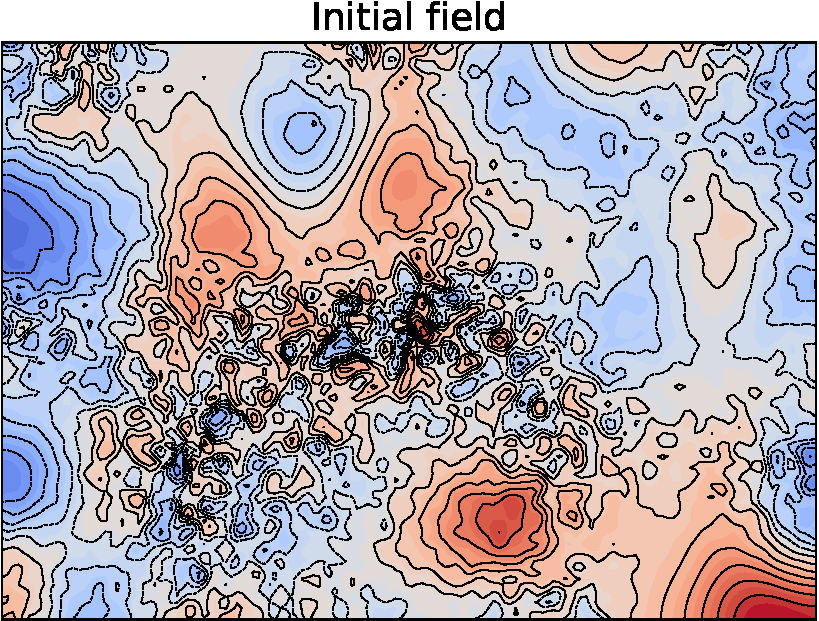
\includegraphics[width=0.49\linewidth]{init.pdf}
\captionof{figure}{Random field with different scales depending on the location. \label{fig:init}}
\end{center}

\begin{center}
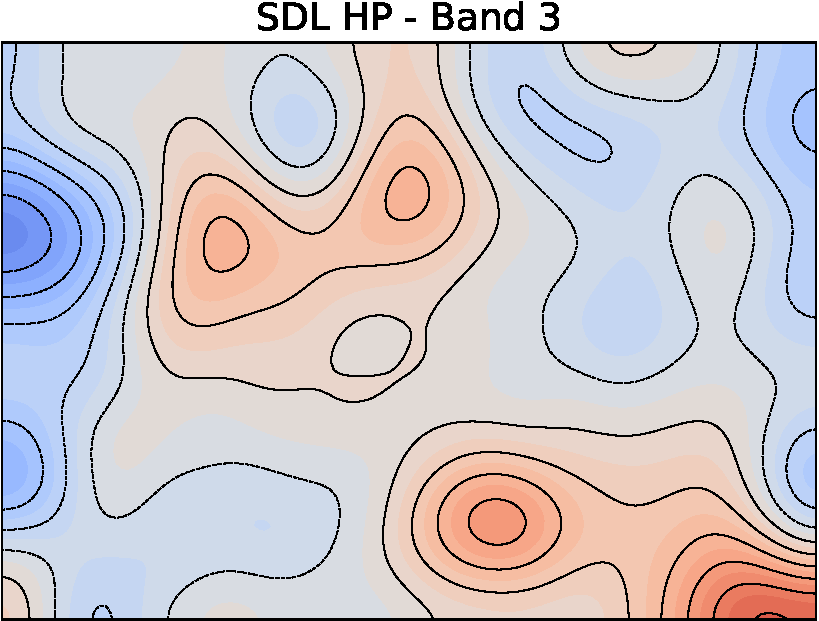
\includegraphics[width=0.49\linewidth]{sdl_hp_band_3.pdf}
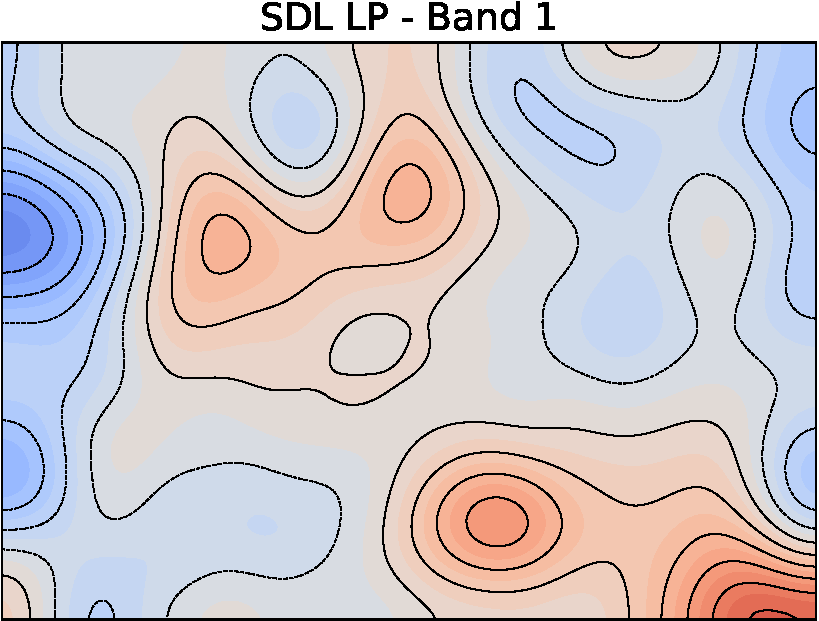
\includegraphics[width=0.49\linewidth]{sdl_lp_band_1.pdf}
\captionof{figure}{Largest scale band for low-pass (left) and high-pass (right) filters. \label{fig:band_large}}
\end{center}

\begin{center}
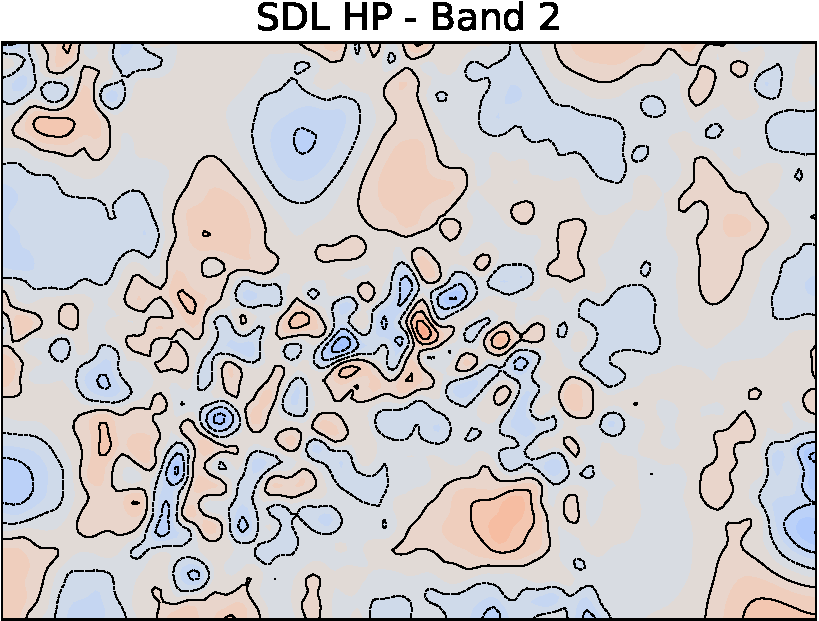
\includegraphics[width=0.49\linewidth]{sdl_hp_band_2}
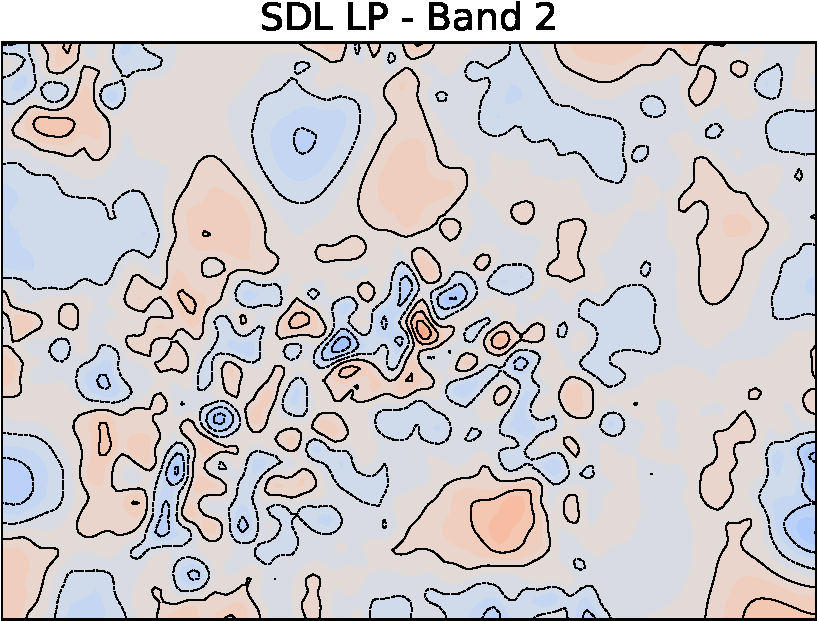
\includegraphics[width=0.49\linewidth]{sdl_lp_band_2.pdf}
\captionof{figure}{Intermediate scale band for low-pass (left) and high-pass (right) filters. \label{fig:band_inter}}
\end{center}

\begin{center}
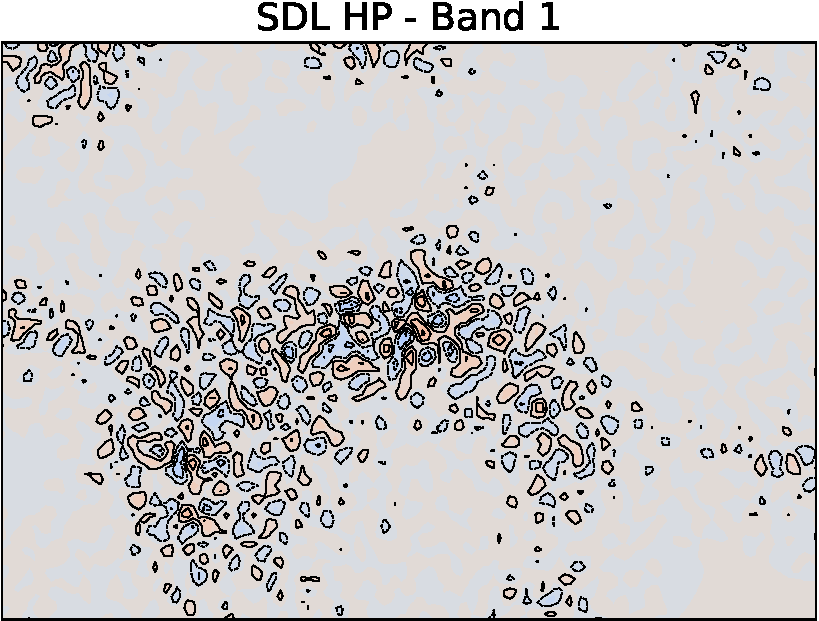
\includegraphics[width=0.49\linewidth]{sdl_hp_band_1.pdf}
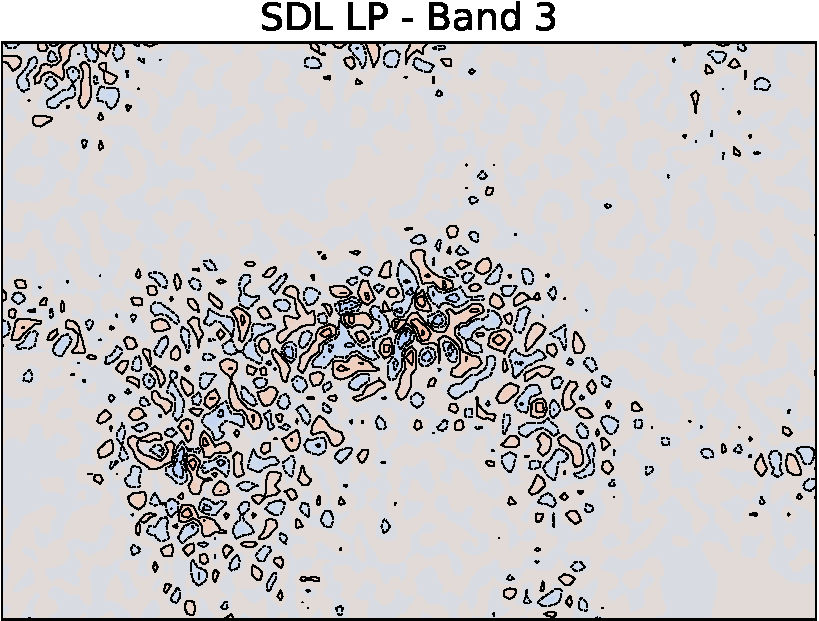
\includegraphics[width=0.49\linewidth]{sdl_lp_band_3.pdf}
\captionof{figure}{Smallest scale band for low-pass (left) and high-pass (right) filters. \label{fig:band_small}}
\end{center}



\subsection{Application}

The standard scale-dependent localization (SDL) described in \citet{buehner_2015b} is a case where the band-pass filters are:
\begin{itemize}
\item either defined explicitely in spectral space, in a "wavelet-like" fashion,
\item or built recursively from high-pass filters, themselves implemented as complements of diffusion-based low-pass filters.
\end{itemize}
$  $\\
However, Figure \ref{fig:} shows that 



% Bibliography
\bibliographystyle{mybib-en}
\bibliography{filter_banks_localization}
\end{document}



\end{document}

The interpolation-based filter banks localization (ILPFL) is a special case of a construction with filter banks localization (FBL) where the low-pass filter $\mathbf{G}_p$ for component $p$ is given by:
\begin{align}
\mathbf{G}_p = \mathbf{N}_p \mathbf{S}_p^\mathrm{T}
\end{align}
where the i$^\text{th}$ coefficient of the diagonal normalization matrix $\mathbf{N}_p$ is equal to the inverse of the i$^\text{th}$ coefficient of the vector $\mathbf{S}_p^\mathrm{T} \mathbf{1}_n$.

\subsection{Methods comparison}
To illustrate the similarities and differences between the SDL and IFBL methods, we start from a random field $\mathbf{x}$ with different scales depending on the location in Figure \ref{fig:init}. In Figure \ref{fig:filt_1}, the filtered field $\widehat{\mathbf{x}}_1$ at low resolution captures the largest scales of the signal. These scales are removed in the corresponding residual $\overline{\mathbf{x}}_1$, in Figure \ref{fig:res_1}. In Figure \ref{fig:filt_2}, the filtered field $\widehat{\mathbf{x}}_2$ at intermediate resolution captures the intermediate scales of the signal. Only the smallest scale are left in the final residual $\overline{\mathbf{x}}_2$, in Figure \ref{fig:res_2}.\\
$  $\\
Here, the SDL uses the \texttt{scipy.ndimage.gaussian\_filter} function of \texttt{Python} for $\mathbf{G}_p$. The IFBL uses a standard bilinear interpolation. The filtering scales of the SDL and the low-resolution grids of the IFBL have been briefly tuned to yield visually similar results.

\begin{center}
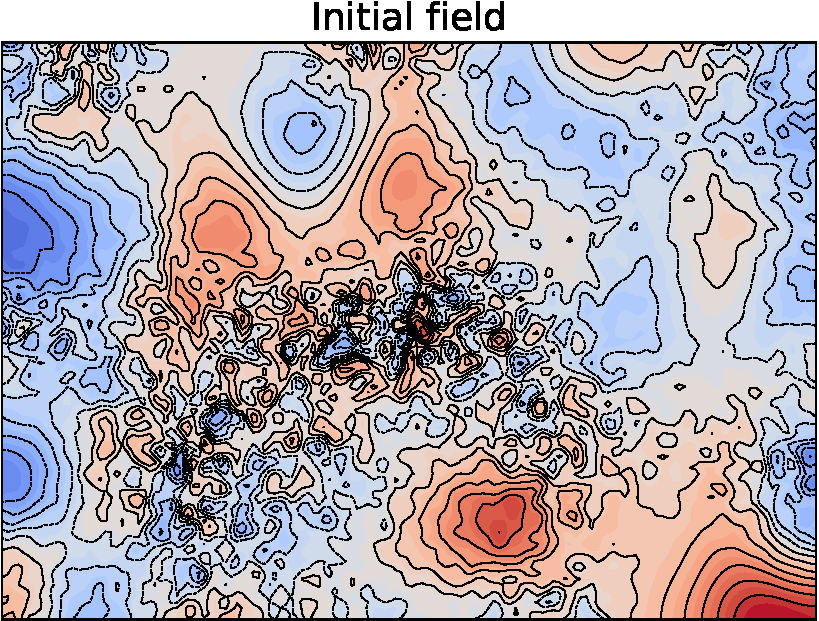
\includegraphics[width=0.49\linewidth]{init.pdf}
\captionof{figure}{Random field with different scales depending on the location. \label{fig:init}}
\end{center}

\begin{center}
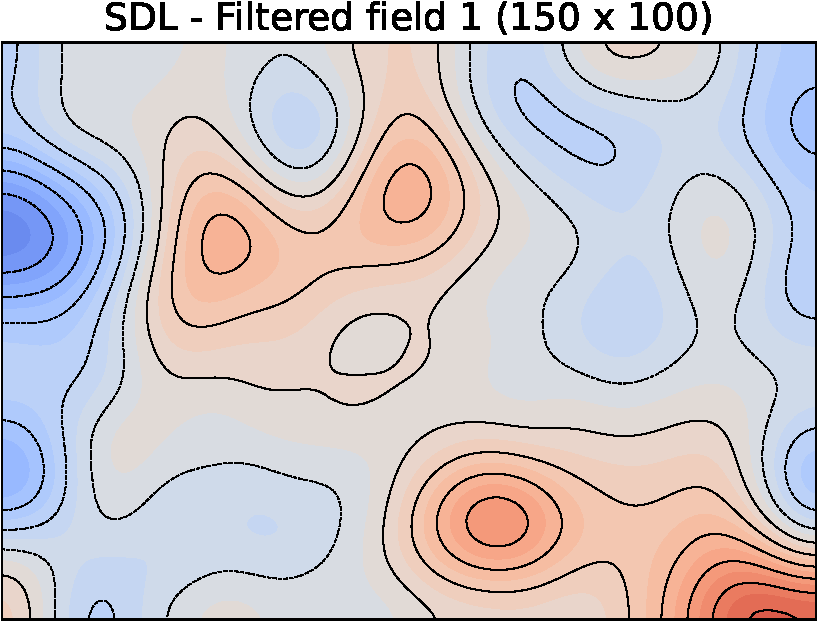
\includegraphics[width=0.49\linewidth]{sdl_1_filt.pdf}
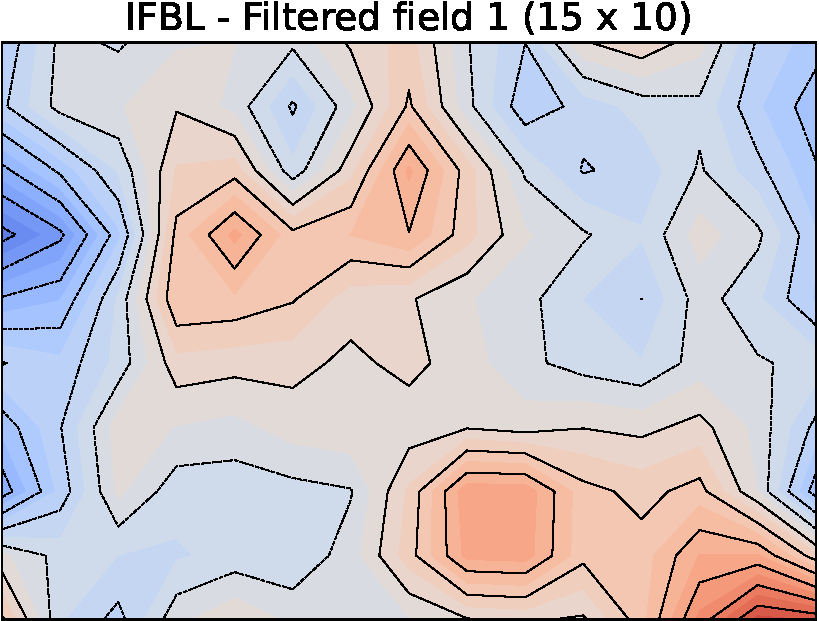
\includegraphics[width=0.49\linewidth]{ifbl_1_filt.pdf}
\captionof{figure}{Filtered field at low-resolution 1 with SDL (left) and IFBL (right)and corresponding residual (right). \label{fig:filt_1}}
\end{center}

\begin{center}
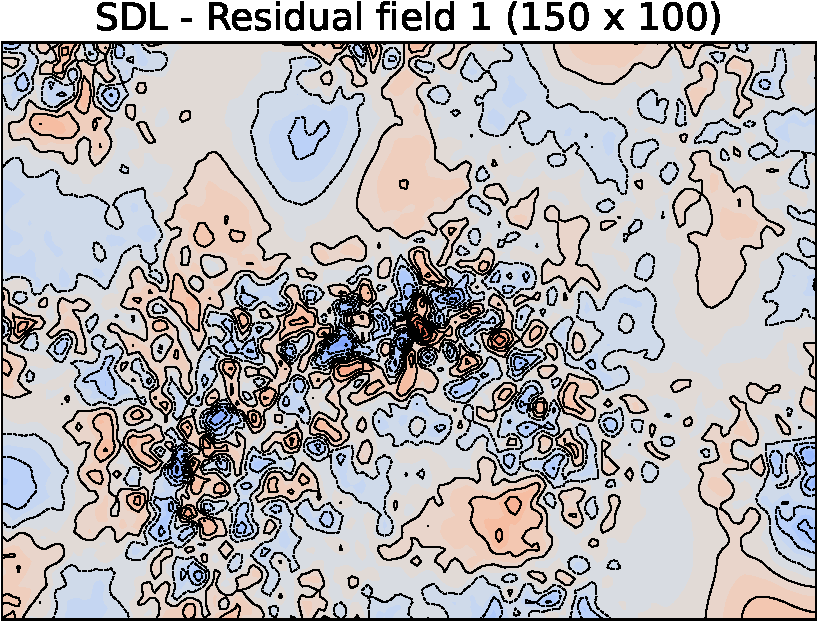
\includegraphics[width=0.49\linewidth]{sdl_1_res.pdf}
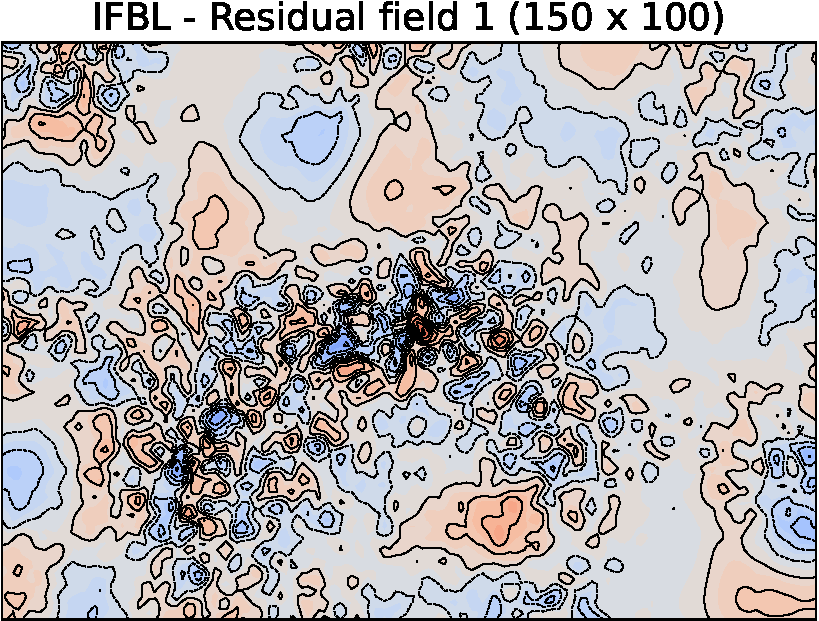
\includegraphics[width=0.49\linewidth]{ifbl_1_res.pdf}
\captionof{figure}{Residual field at low-resolution 1 with SDL (left) and IFBL (right). \label{fig:res_1}}
\end{center}

\begin{center}
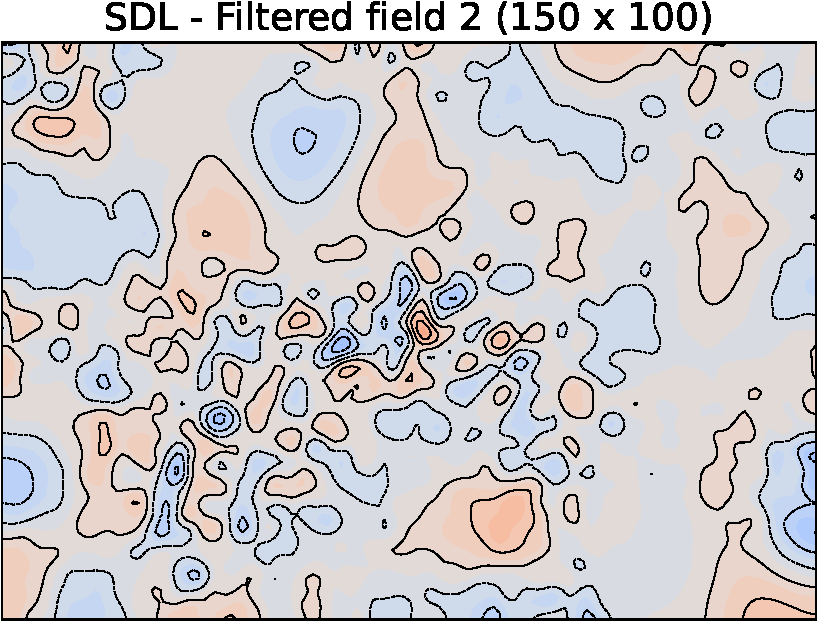
\includegraphics[width=0.49\linewidth]{sdl_2_filt.pdf}
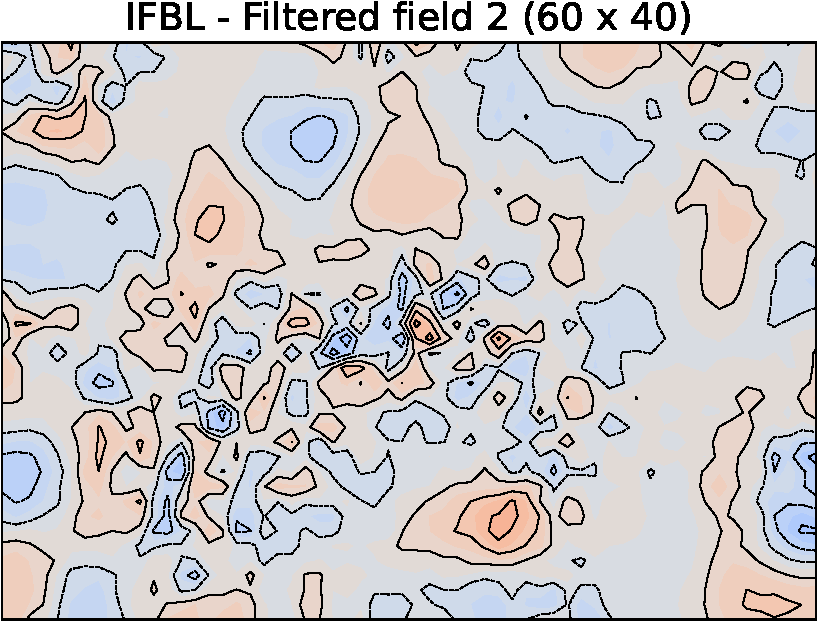
\includegraphics[width=0.49\linewidth]{ifbl_2_filt.pdf}
\captionof{figure}{Filtered field at low-resolution 2 with SDL (left) and IFBL (right)and corresponding residual (right). \label{fig:filt_2}}
\end{center}

\begin{center}
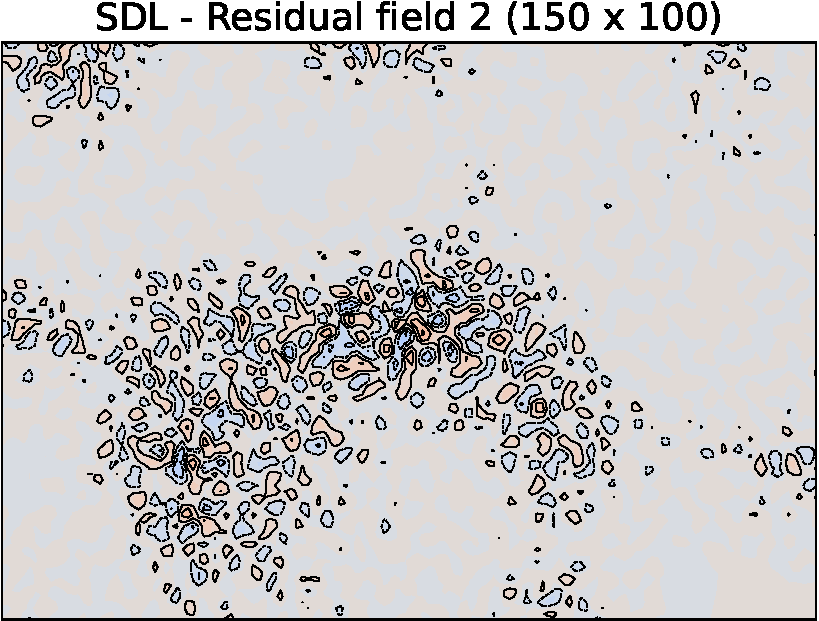
\includegraphics[width=0.49\linewidth]{sdl_2_res.pdf}
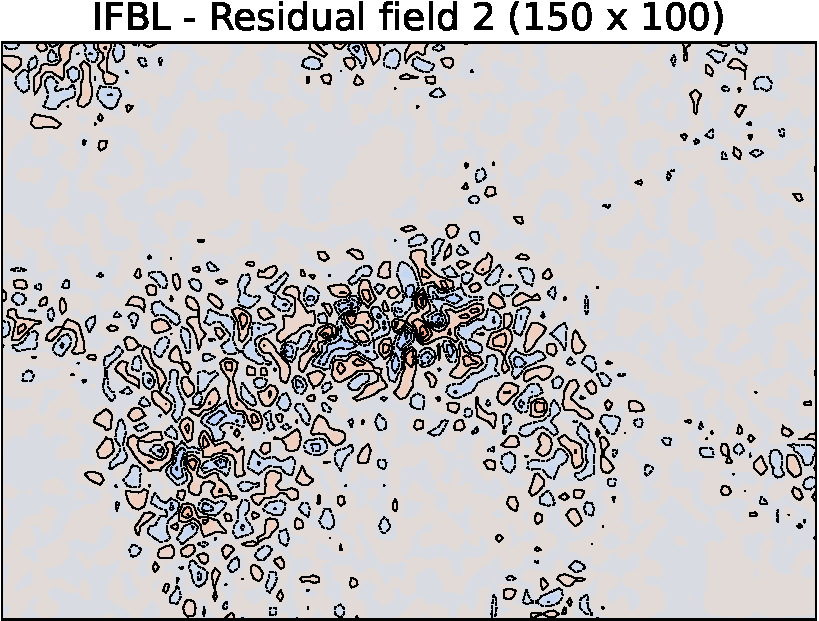
\includegraphics[width=0.49\linewidth]{ifbl_2_res.pdf}
\captionof{figure}{Residual field at low-resolution 2 with SDL (left) and IFBL (right). \label{fig:res_2}}
\end{center}

The interpolation-based filter banks localization (IFBL) leads to a smaller size of the transformed space $\widehat{n}$ than the scale-dependent localization (SDL), reducing the required memory for the same number of components. Also, the choice of the grids for the low-resolution components is completely flexible. Once the interpolation from low resolution to full resolution and its adjoint are available, the construction of the low-pass filter is straightforward. However, the IFBL requires that the localization matrix is applied in the geoemetry of each component, which is more complicated but also cheaper because the localization is applied at lower resolution.

% Bibliography
\bibliographystyle{mybib-en}
\bibliography{filter_banks_localization}
\end{document}
